% Options for packages loaded elsewhere
\PassOptionsToPackage{unicode}{hyperref}
\PassOptionsToPackage{hyphens}{url}
%
\documentclass[
  doc, donotrepeattitle,floatsintext]{apa7}
\usepackage{amsmath,amssymb}
\usepackage{lmodern}
\usepackage{iftex}
\ifPDFTeX
  \usepackage[T1]{fontenc}
  \usepackage[utf8]{inputenc}
  \usepackage{textcomp} % provide euro and other symbols
\else % if luatex or xetex
  \usepackage{unicode-math}
  \defaultfontfeatures{Scale=MatchLowercase}
  \defaultfontfeatures[\rmfamily]{Ligatures=TeX,Scale=1}
\fi
% Use upquote if available, for straight quotes in verbatim environments
\IfFileExists{upquote.sty}{\usepackage{upquote}}{}
\IfFileExists{microtype.sty}{% use microtype if available
  \usepackage[]{microtype}
  \UseMicrotypeSet[protrusion]{basicmath} % disable protrusion for tt fonts
}{}
\makeatletter
\@ifundefined{KOMAClassName}{% if non-KOMA class
  \IfFileExists{parskip.sty}{%
    \usepackage{parskip}
  }{% else
    \setlength{\parindent}{0pt}
    \setlength{\parskip}{6pt plus 2pt minus 1pt}}
}{% if KOMA class
  \KOMAoptions{parskip=half}}
\makeatother
\usepackage{xcolor}
\usepackage{graphicx}
\makeatletter
\def\maxwidth{\ifdim\Gin@nat@width>\linewidth\linewidth\else\Gin@nat@width\fi}
\def\maxheight{\ifdim\Gin@nat@height>\textheight\textheight\else\Gin@nat@height\fi}
\makeatother
% Scale images if necessary, so that they will not overflow the page
% margins by default, and it is still possible to overwrite the defaults
% using explicit options in \includegraphics[width, height, ...]{}
\setkeys{Gin}{width=\maxwidth,height=\maxheight,keepaspectratio}
% Set default figure placement to htbp
\makeatletter
\def\fps@figure{htbp}
\makeatother
\setlength{\emergencystretch}{3em} % prevent overfull lines
\providecommand{\tightlist}{%
  \setlength{\itemsep}{0pt}\setlength{\parskip}{0pt}}
\setcounter{secnumdepth}{-\maxdimen} % remove section numbering
% Make \paragraph and \subparagraph free-standing
\ifx\paragraph\undefined\else
  \let\oldparagraph\paragraph
  \renewcommand{\paragraph}[1]{\oldparagraph{#1}\mbox{}}
\fi
\ifx\subparagraph\undefined\else
  \let\oldsubparagraph\subparagraph
  \renewcommand{\subparagraph}[1]{\oldsubparagraph{#1}\mbox{}}
\fi
\newlength{\cslhangindent}
\setlength{\cslhangindent}{1.5em}
\newlength{\csllabelwidth}
\setlength{\csllabelwidth}{3em}
\newlength{\cslentryspacingunit} % times entry-spacing
\setlength{\cslentryspacingunit}{\parskip}
\newenvironment{CSLReferences}[2] % #1 hanging-ident, #2 entry spacing
 {% don't indent paragraphs
  \setlength{\parindent}{0pt}
  % turn on hanging indent if param 1 is 1
  \ifodd #1
  \let\oldpar\par
  \def\par{\hangindent=\cslhangindent\oldpar}
  \fi
  % set entry spacing
  \setlength{\parskip}{#2\cslentryspacingunit}
 }%
 {}
\usepackage{calc}
\newcommand{\CSLBlock}[1]{#1\hfill\break}
\newcommand{\CSLLeftMargin}[1]{\parbox[t]{\csllabelwidth}{#1}}
\newcommand{\CSLRightInline}[1]{\parbox[t]{\linewidth - \csllabelwidth}{#1}\break}
\newcommand{\CSLIndent}[1]{\hspace{\cslhangindent}#1}
\ifLuaTeX
\usepackage[bidi=basic]{babel}
\else
\usepackage[bidi=default]{babel}
\fi
\babelprovide[main,import]{english}
% get rid of language-specific shorthands (see #6817):
\let\LanguageShortHands\languageshorthands
\def\languageshorthands#1{}
% Manuscript styling
\usepackage{upgreek}
\captionsetup{font=singlespacing,justification=justified}

% Table formatting
\usepackage{longtable}
\usepackage{lscape}
% \usepackage[counterclockwise]{rotating}   % Landscape page setup for large tables
\usepackage{multirow}		% Table styling
\usepackage{tabularx}		% Control Column width
\usepackage[flushleft]{threeparttable}	% Allows for three part tables with a specified notes section
\usepackage{threeparttablex}            % Lets threeparttable work with longtable

% Create new environments so endfloat can handle them
% \newenvironment{ltable}
%   {\begin{landscape}\centering\begin{threeparttable}}
%   {\end{threeparttable}\end{landscape}}
\newenvironment{lltable}{\begin{landscape}\centering\begin{ThreePartTable}}{\end{ThreePartTable}\end{landscape}}

% Enables adjusting longtable caption width to table width
% Solution found at http://golatex.de/longtable-mit-caption-so-breit-wie-die-tabelle-t15767.html
\makeatletter
\newcommand\LastLTentrywidth{1em}
\newlength\longtablewidth
\setlength{\longtablewidth}{1in}
\newcommand{\getlongtablewidth}{\begingroup \ifcsname LT@\roman{LT@tables}\endcsname \global\longtablewidth=0pt \renewcommand{\LT@entry}[2]{\global\advance\longtablewidth by ##2\relax\gdef\LastLTentrywidth{##2}}\@nameuse{LT@\roman{LT@tables}} \fi \endgroup}

% \setlength{\parindent}{0.5in}
% \setlength{\parskip}{0pt plus 0pt minus 0pt}

% Overwrite redefinition of paragraph and subparagraph by the default LaTeX template
% See https://github.com/crsh/papaja/issues/292
\makeatletter
\renewcommand{\paragraph}{\@startsection{paragraph}{4}{\parindent}%
  {0\baselineskip \@plus 0.2ex \@minus 0.2ex}%
  {-1em}%
  {\normalfont\normalsize\bfseries\itshape\typesectitle}}

\renewcommand{\subparagraph}[1]{\@startsection{subparagraph}{5}{1em}%
  {0\baselineskip \@plus 0.2ex \@minus 0.2ex}%
  {-\z@\relax}%
  {\normalfont\normalsize\itshape\hspace{\parindent}{#1}\textit{\addperi}}{\relax}}
\makeatother

% \usepackage{etoolbox}
\makeatletter
\patchcmd{\HyOrg@maketitle}
  {\section{\normalfont\normalsize\abstractname}}
  {\section*{\normalfont\normalsize\abstractname}}
  {}{\typeout{Failed to patch abstract.}}
\patchcmd{\HyOrg@maketitle}
  {\section{\protect\normalfont{\@title}}}
  {\section*{\protect\normalfont{\@title}}}
  {}{\typeout{Failed to patch title.}}
\makeatother

\usepackage{xpatch}
\makeatletter
\xapptocmd\appendix
  {\xapptocmd\section
    {\addcontentsline{toc}{section}{\appendixname\ifoneappendix\else~\theappendix\fi\\: #1}}
    {}{\InnerPatchFailed}%
  }
{}{\PatchFailed}
\usepackage{csquotes}
\usepackage{pdflscape}
\usepackage{setspace}
\raggedbottom
\AtBeginDocument{\let\maketitle\relax}
\renewcommand{\thefigure}{S\arabic{figure}} \setcounter{figure}{0}
\renewcommand{\thetable}{S\arabic{table}} \setcounter{table}{0}
\ifLuaTeX
  \usepackage{selnolig}  % disable illegal ligatures
\fi
\IfFileExists{bookmark.sty}{\usepackage{bookmark}}{\usepackage{hyperref}}
\IfFileExists{xurl.sty}{\usepackage{xurl}}{} % add URL line breaks if available
\urlstyle{same} % disable monospaced font for URLs
\hypersetup{
  pdftitle={Exercising choice over feedback schedules during practice is not advantageous for motor learning},
  pdflang={en-EN},
  hidelinks,
  pdfcreator={LaTeX via pandoc}}

\title{Exercising choice over feedback schedules during practice is not advantageous for motor learning}
\author{\phantom{0}}
\date{}


\shorttitle{Choice and feedback characteristics}

\affiliation{\phantom{0}}

\begin{document}
\maketitle

\hypertarget{supplementary-a}{%
\section{Supplementary A}\label{supplementary-a}}

Model diagnostics of total error (E) for the spatial and timing goals revealed skewed distributions. As a result, we carried out sensitivity analyses using shift functions, which is a robust technique that is well-suited for skewed distributions (Rousselet \& Wilcox, 2020; Wilcox, 2021). For all shift functions, we collapsed across retention and transfer data to compute a single post-test score for both the spatial and timing goals. Given our primary interest was related to the role of choice during practice for motor learning and shift functions only compare two groups, we only ran these analyses on the choice factor for Experiment 1 (collapsed across feedback) and Experiment 2. Conducting a shift function analysis is a multi-step process that first involved calculating the 20\% trimmed means for each participant and time point. Next, deciles for the factor of choice (choice versus yoked) in Experiments 1 and 2 were calculated using the Harrell-Davis estimator (Harrell \& Davis, 1982; Rousselet et al., 2017). Lastly, differences at each decile were evaluated based on the 95\% confidence intervals corrected for multiple comparisons using Hochberg's method (Hochberg, 1988). Spatial and timing measures were analyzed separately for Experiments 1 and 2.

\hypertarget{choice-versus-yoked}{%
\subsection{Choice versus yoked}\label{choice-versus-yoked}}

For Experiment 1, the 95\% confidence intervals overlapped with zero at each decile when comparing the choice and yoked groups for both the spatial (Fig. \ref{fig:figS1}A) and timing (Fig. \ref{fig:figS2}A) goals. Similarly, in Experiment 2 there were no significant differences between the choice and yoked groups in any decile for the spatial (Fig. \ref{fig:figS1}B) and timing (Fig. \ref{fig:figS2}B) goals. The results from these shift function analyses are consistent with the analyses reported in the main manuscript and a recent meta-analysis (McKay et al., in-press), suggesting that giving learners choice during practice is not advantageous for motor learning.

\begin{figure}

{\centering 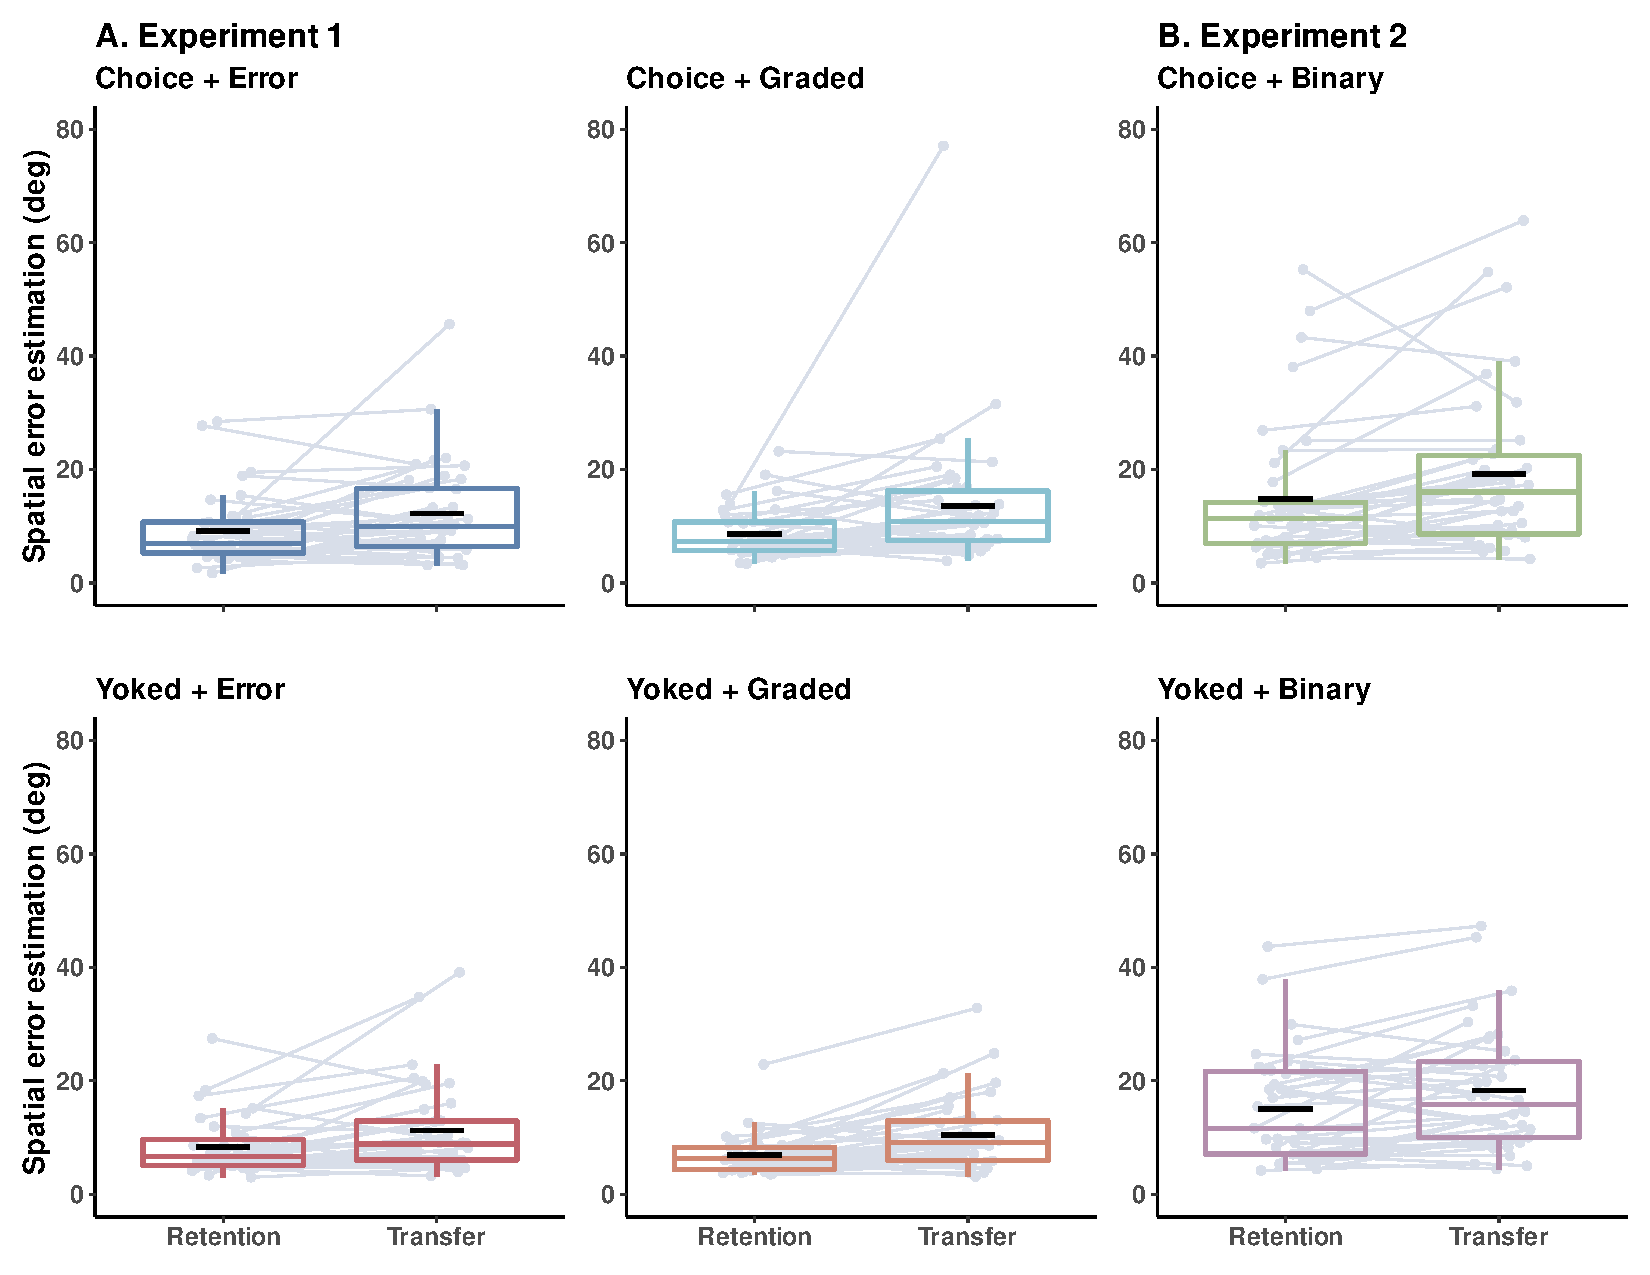
\includegraphics{../../figs/figS1} 

}

\caption{\small \normalfont \onehalfspacing \textbf{Post-test (collapsed across retention and transfer) spatial E (deg) shift function.} The top row illustrates scatter plots of individual mean spatial E for each group in Experiment 1 \textbf{(A)} and Experiment 2 \textbf{(B)}. The middle row illustrates the same scatter plots as the top row, but with the deciles of each distribution represented by the black lines. The thick black line represents the the median of each distribution. The deciles from each group are joined by colored lines, with blue (Experiment 1) and green (Experiment 2) indicating lower error for the choice group deciles, and red (Experiment 1) and green (Experiment 2) indicating lower error for the yoked group deciles. The bottom row illustrates the shift function, which focuses on the grey shaded region of the x-axis in the middle row. The deciles for the choice group are plotted on the x-axis and the difference in deciles between the choice and yoked group are plotted on the y-axis. The vertical dash line represents the median of the choice distribution. The same color coding for differences in deciles from the middle row is used in the bottom row. Error bars represent 95\% confidence intervals, corrected for multiple comparisons. The horizontal dashed line represents zero differences between the deciles of the two group. If a 95\% confidence interval overlaps with zero, there is no significant difference between the two groups on that decile of the distribution. There were no significant differences for any decile in either experiment.}\label{fig:figS1}
\end{figure}



\begin{figure}

{\centering 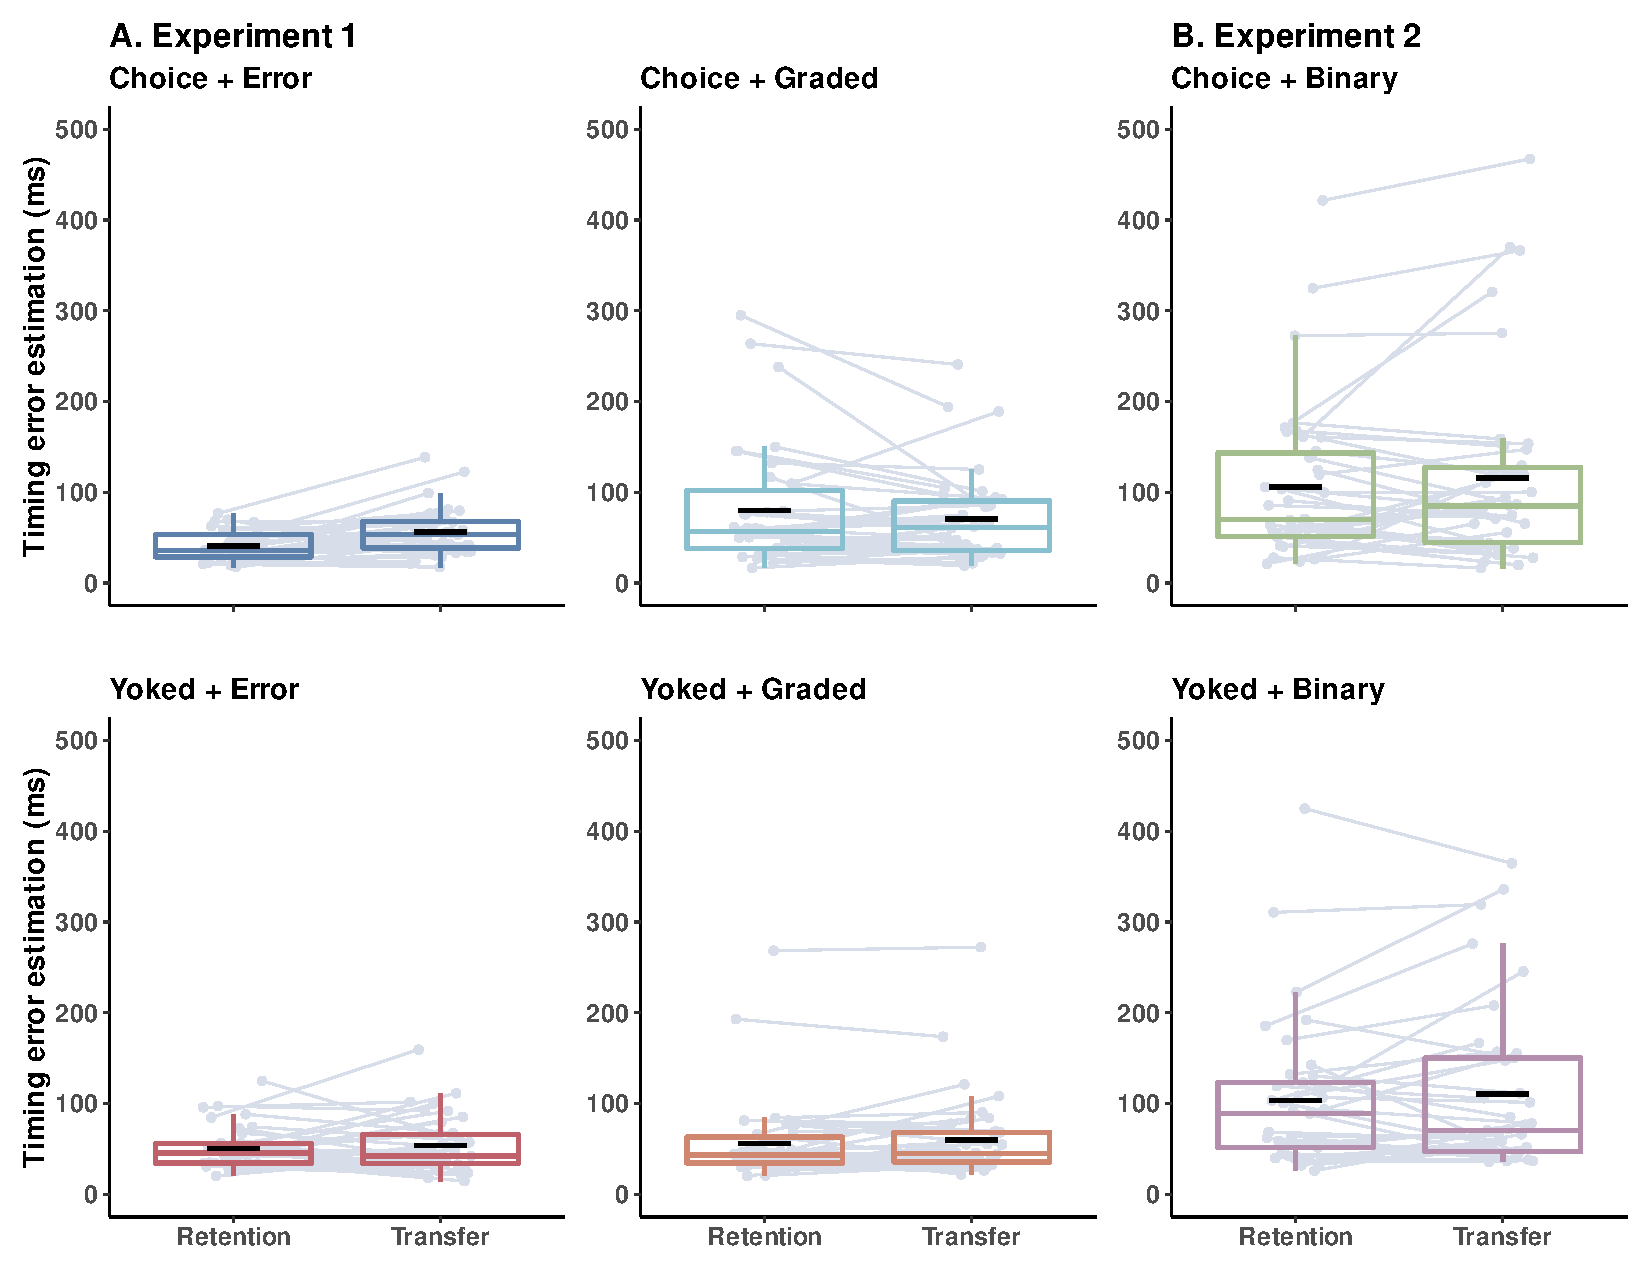
\includegraphics{../../figs/figS2} 

}

\caption{\small \normalfont \onehalfspacing \textbf{Post-test (collapsed across retention and transfer) timing E (ms) shift function.} The top row illustrates scatter plots of individual mean timing E for each group in Experiment 1 \textbf{(A)} and Experiment 2 \textbf{(B)}. The middle row illustrates the same scatter plots as the top row, but with the deciles of each distribution represented by the black lines. The thick black line represents the the median of each distribution. The deciles from each group are joined by colored lines, with blue (Experiment 1) and green (Experiment 2) indicating lower error for the choice group deciles, and red (Experiment 1) and green (Experiment 2) indicating lower error for the yoked group deciles. The bottom row illustrates the shift function, which focuses on the grey shaded region of the x-axis in the middle row. The deciles for the choice group are plotted on the x-axis and the difference in deciles between the choice and yoked group are plotted on the y-axis. The vertical dash line represents the median of the choice distribution. The same color coding for differences in deciles from the middle row is used in the bottom row. Error bars represent 95\% confidence intervals, corrected for multiple comparisons. The horizontal dashed line represents zero differences between the deciles of the two group. If a 95\% confidence interval overlaps with zero, there is no significant difference between the two groups on that decile of the distribution. There were no significant differences for any decile in either experiment.}\label{fig:figS2}
\end{figure}



\clearpage

\hypertarget{supplementary-b}{%
\section{Supplementary B}\label{supplementary-b}}

We asked all participants to estimate their performance on the spatial (Fig. \ref{fig:figS3}) and timing (Fig. \ref{fig:figS4}) components of the motor task after each trial in retention and transfer, similar to past research (e.g., Barros et al., 2019; Carter et al., 2014; Carter \& Patterson, 2012). Additionally, half of the participants in each group were randomly selected to also estimate their performance after each trial in the pre-test (not shown). To assess error estimation for the spatial and timing components, we first calculated the difference between a participant's estimated performance and their actual performance on each trial. Next, we computed total estimation error (EE) using the equation:
\begin{equation}
EE = \sqrt{CE^2 + VE^2}
\end{equation}
where \(CE\) was the average estimation bias and \(VE\) was the standard deviation of these errors. This approach is consistent with that used by Bruechert et al. (2003).

\hypertarget{error-estimation-in-retention-and-transfer}{%
\subsection{Error estimation in retention and transfer}\label{error-estimation-in-retention-and-transfer}}

Total estimation error was generally lower in retention compared to transfer for both the spatial (Fig. \ref{fig:figS3}) and timing (Fig. \ref{fig:figS4}) domains in Experiments 1 and 2. For the spatial estimation error, we found a significant main effect of Test in Experiment 1, \(F(1,148) = 32.40\), \(p < .001\), \(\eta_{G}^2 = .060\), and in Experiment 2, \(F(1,74) = 18.79\), \(p < .001\), \(\eta_{G}^2 = .026\), with more accurate estimations in retention than transfer. Although there was a significant Choice x Feedback x Test interaction in Experiment 1 for timing estimation error, \(F(1,148) = 7.12\), \(p = .008\), \(\eta_{G}^2 < .001\), we did not decompose the interaction as the effect size estimate was less than \(.001\). There were no significant main effects or interactions for timing estimation error in Experiment 2. A potential explanation for the difference in estimation accuracy between retention and transfer for the spatial component and not the the timing component is that only the spatial goal changed. Specifically, it was 40 deg in retention and 60 deg in transfer whereas the timing goal remained 225 ms in both tests.

\clearpage

\begin{figure}

{\centering 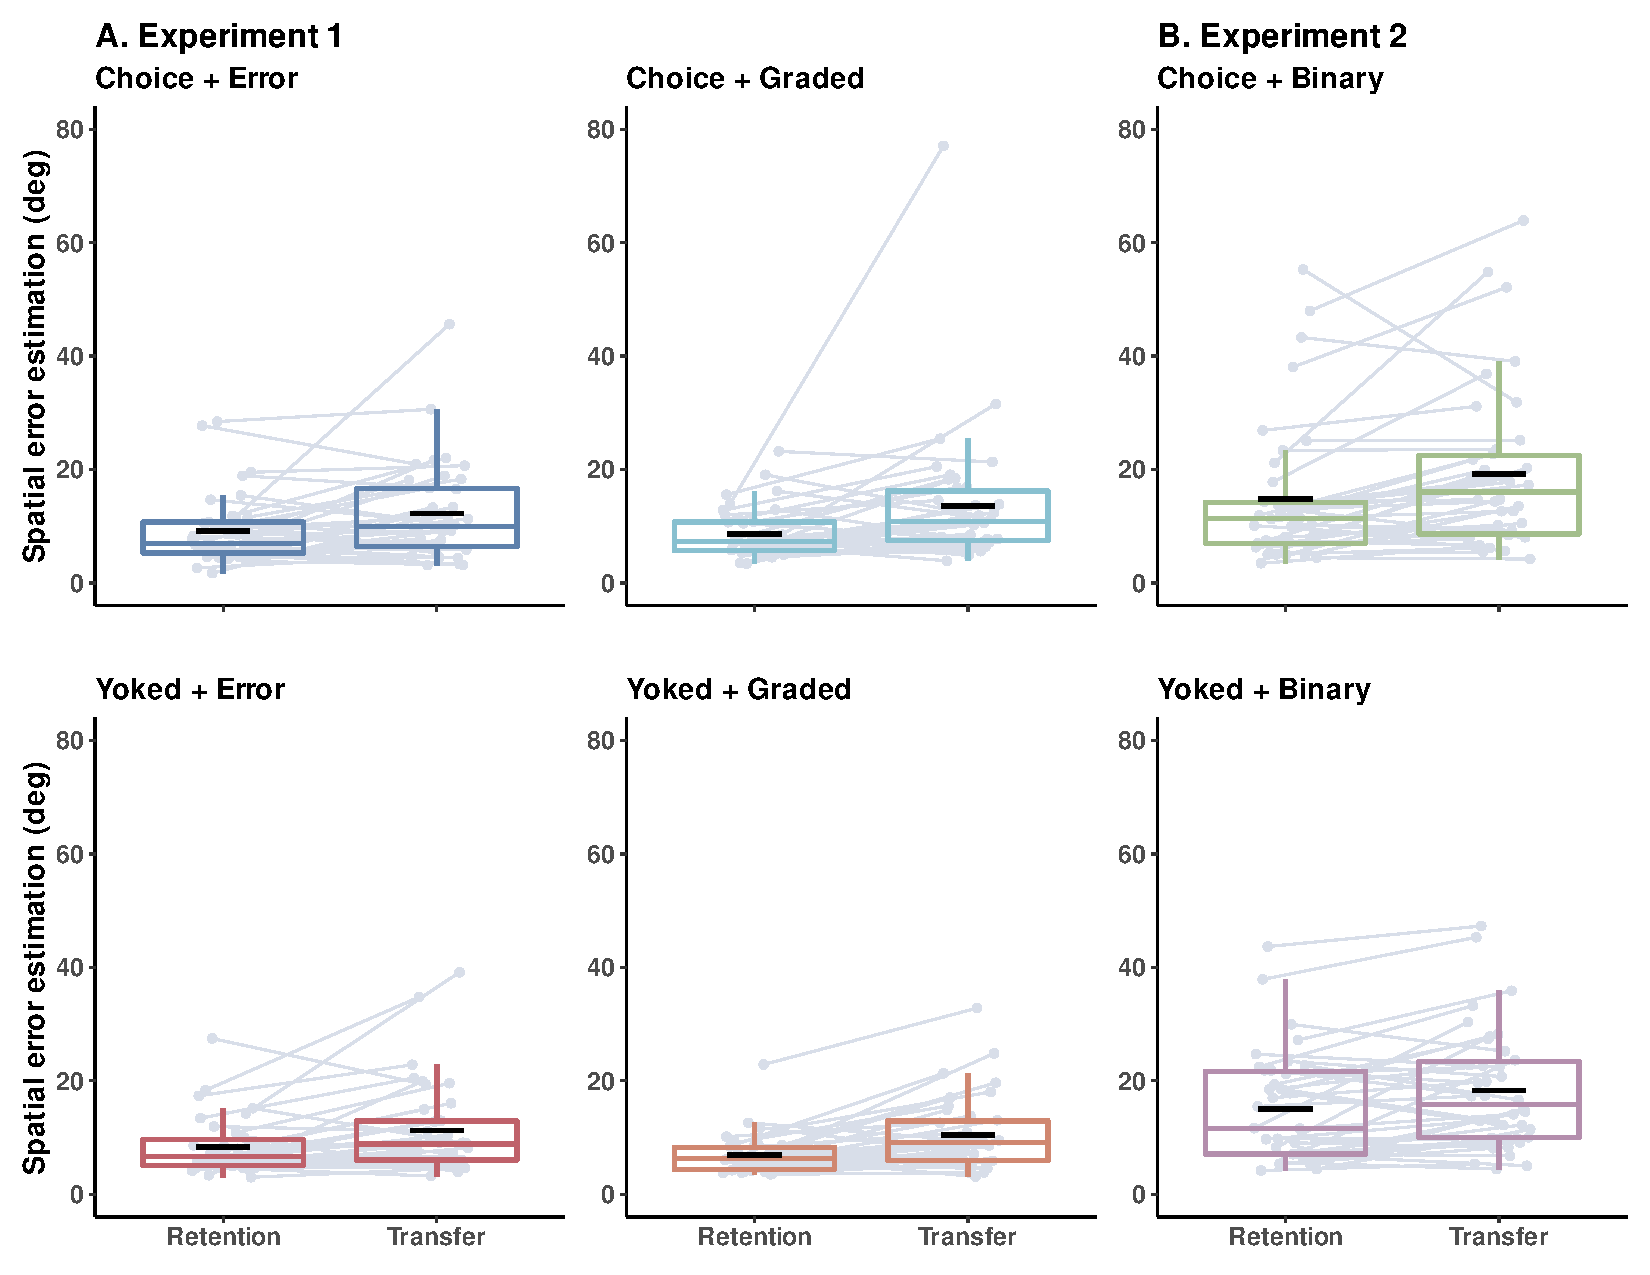
\includegraphics{../../figs/figS3} 

}

\caption{\small \normalfont \onehalfspacing \textbf{Total spatial error estimation data.} Boxplots of retention and transfer data from all participants for Experiment 1 \textbf{(A)} and Experiment 2 \textbf{(B)}. The Choice with error feedback (Choice+Error) group is shown in dark blue, the Choice with graded feedback (Choice+Graded) group is shown in light blue, the Choice with binary feedback (Choice+Binary) group is shown in green, the Yoked with error feedback (Yoked+Error) group is shown in red, the Yoked with graded feedback (Yoked+Graded) group is shown in yellow, and the Yoked with binary feedback (Yoked+Binary) group is shown in purple. Boxplots represent 25th, 50th, and 75th percentiles, and the solid black line denotes the group mean. Grey connected dots represent individual data for participants in each group.}\label{fig:figS3}
\end{figure}



\begin{figure}

{\centering 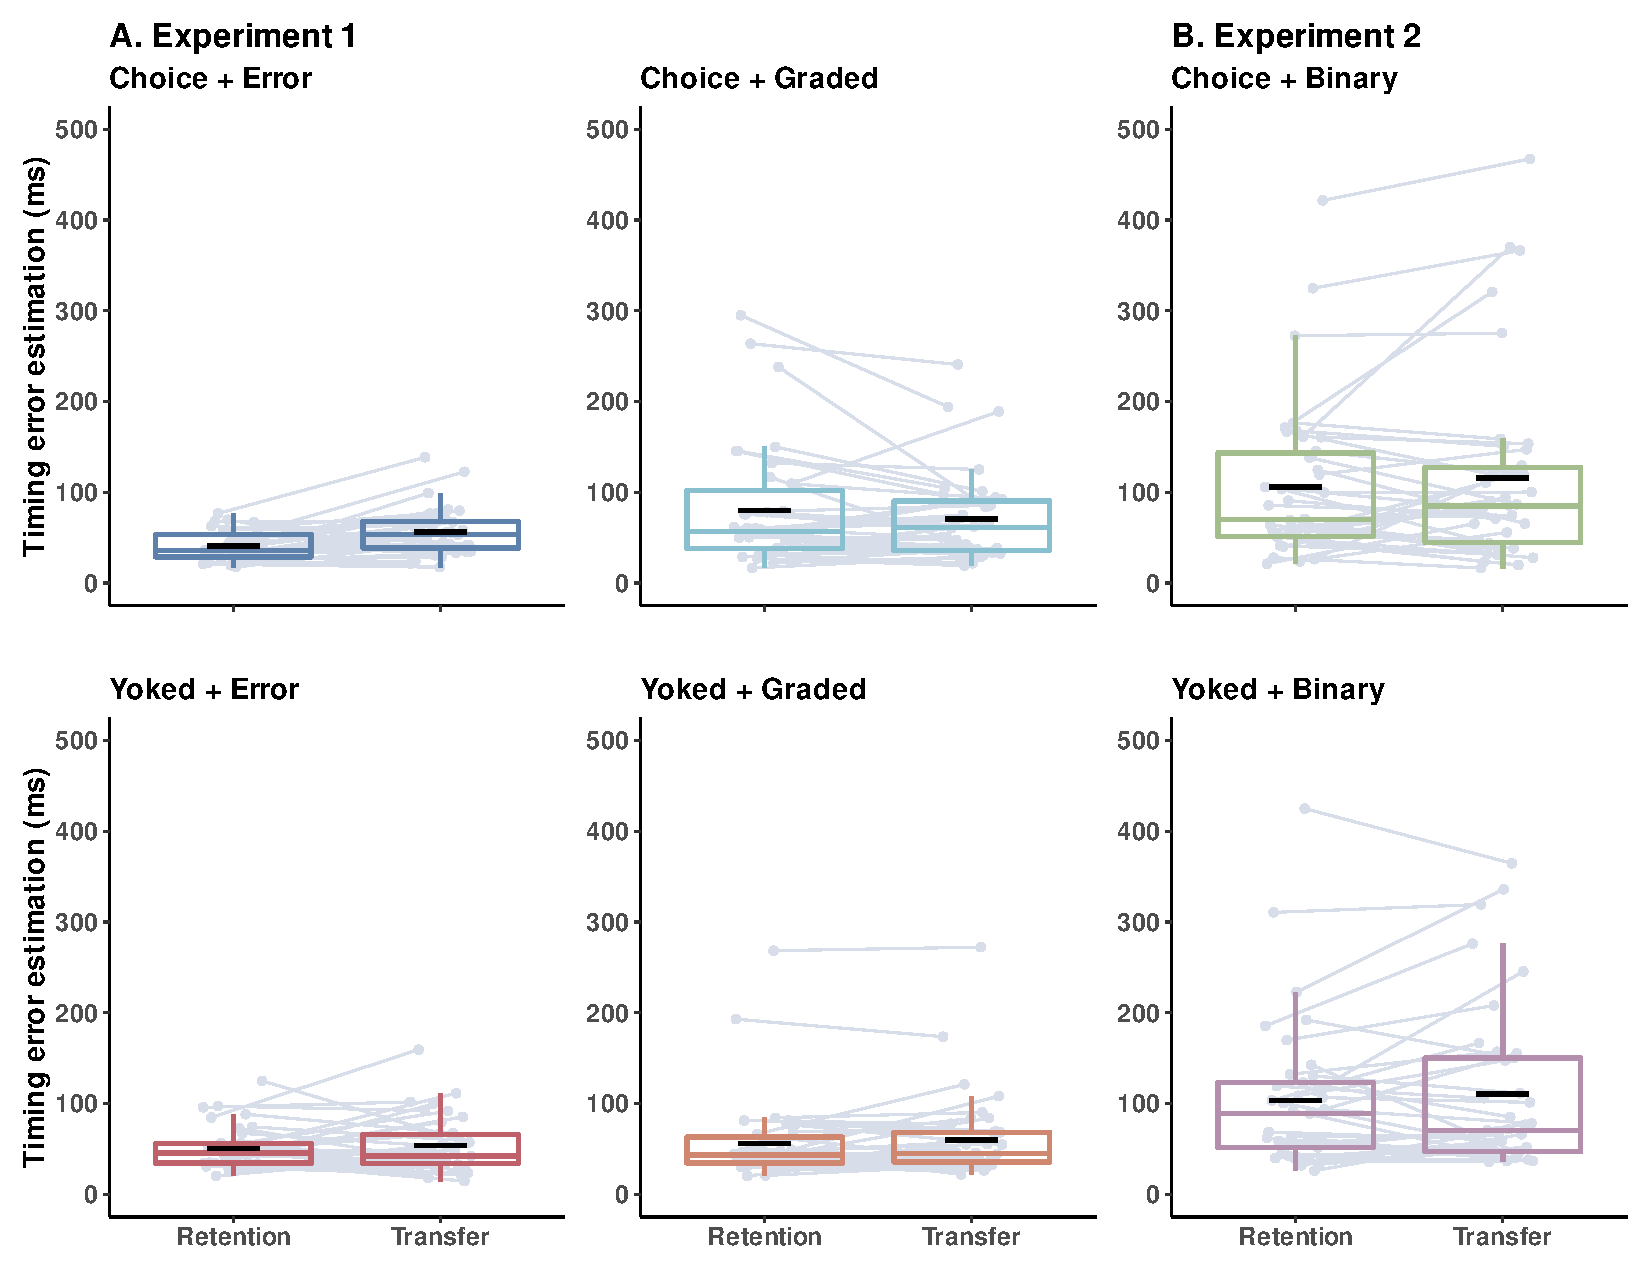
\includegraphics{../../figs/figS4} 

}

\caption{\small \normalfont \onehalfspacing \textbf{Total timing error estimation data.} Boxplots of retention and transfer data from all participants for Experiment 1 \textbf{(A)} and Experiment 2 \textbf{(B)}. The Choice with error feedback (Choice+Error) group is shown in dark blue, the Choice with graded feedback (Choice+Graded) group is shown in light blue, the Choice with binary feedback (Choice+Binary) group is shown in green, the Yoked with error feedback (Yoked+Error) group is shown in red, the Yoked with graded feedback (Yoked+Graded) group is shown in yellow, and the Yoked with binary feedback (Yoked+Binary) group is shown in purple. Boxplots represent 25th, 50th, and 75th percentiles, and the solid black line denotes the group mean. Grey connected dots represent individual data for participants in each group. Individual data of 1 participant in each of the Choice+Error, Yoked+Error, and Yoked+Binary groups is not shown as their error exceeded 500 ms.}\label{fig:figS4}
\end{figure}



\clearpage

\hypertarget{development-of-error-estimation-skills}{%
\subsection{Development of error estimation skills}\label{development-of-error-estimation-skills}}

In Experiment 1, the subset of participants in each group who estimated their error after each pre-test trial improved the accuracy of their estimation skills throughout the experiment. We found significant main effects of Test for both the spatial, \(F(1.45,104.67) = 20.72\), \(p < .001\), \(\eta_{G}^2 = .144\), and timing, \(F(1.10,79.40) = 46.88\), \(p < .001\), \(\eta_{G}^2 = .060\), error estimations. For the spatial error estimations, Holm-Bonferonni post-hoc tests revealed that pre-test had higher error than retention and transfer (\(p\)'s \textless{} .001), and transfer had higher error than retention (\(p\) \textless{} .001). Similarly, timing error estimations were more accurate in retention and transfer compared to the pre-test (\(p\)'s \textless{} .001). In Experiment 2, none of the main effects or interactions were significant.

\hypertarget{performance-accuracy-of-estimators-versus-non-estimators}{%
\subsection{Performance accuracy of estimators versus non-estimators}\label{performance-accuracy-of-estimators-versus-non-estimators}}

\textcolor{blue}{We assessed whether performance accuracy differed between the subset of participants who were randomly assigned to estimate their error in pre-test compared to those who were not. Total error for the spatial and timing goals were analyzed in separate mixed ANOVAs (\emph{Acquisition}: 2 Estimation x 6 Block; \emph{Learning}: 2 Estimation x 2 Test) for each experiment. None of the main effect or interactions were significant in Experiment 1 or Experiment 2. A possible explanation for this finding is that estimating one's error is most effective when knowledge of results feedback is provided following the estimation} (Guadagnoli \& Kohl, 2001)\textcolor{blue}{. Another possible explanation is that self-controlled feedback schedules promote spontaneous error estimation} (e.g., Chiviacowsky \& Wulf, 2005). \textcolor{blue}{Given recent support for this idea} (Bacelar et al., 2022)\textcolor{blue}{, it seems plausible that all participants in a self-controlled group in the present experiments engaged is some form of error estimation activities throughout acquisition when they deliberated about using (or not using) one of their limited feedback requests.}

\clearpage

\hypertarget{supplementary-c}{%
\section{Supplementary C}\label{supplementary-c}}

\textcolor{blue}{Contrary to the motivational perspective (i.e., OPTIMAL theory), we did not find that the opportunity to exercise choice over feedback during practice enhanced perceptions of competence, autonomy, or intrinsic motivation relative to not having this same choice opportunity. Equivalence tests can be used to null findings more informative} (Harms \& Lakens, 2018; Lakens, 2017; Schuirmann, 1987)\textcolor{blue}{; however, a typical two one-sided test procedure may not be appropriate for this analysis for a couple reasons. First, we did not specify an \emph{a priori} smallest effect size of interest for any of the psychological constructs. Second, the questionnaires were administered at various time points---after pre-test, after acquisition blocks 1 and 6, and before retention---during the experimental protocol. Given the choice and feedback manipulations were present at after acquisitions blocks 1 and 6 and not after pre-test or before retention, it would be inappropriate to aggregate across time points. We instead report mean differences and 90\% confidence intervals between choice and yoked groups at each questionnaire time point for both experiments. The present experiments can be considered inconsistent with all effects larger than $g = \pm$ the largest absolute confidence interval bound presented in} Table \ref{tab:tableS1}.

\vspace{1em}

\begin{table}[h!]

\caption{\label{tab:tableS1}Effect sizes for each questionnaire at each timepoint.}
\resizebox{\linewidth}{!}{
\fontsize{11}{13}\selectfont
\begin{tabular}[t]{>{\raggedright\arraybackslash}p{11em}>{\raggedright\arraybackslash}p{2em}>{\raggedright\arraybackslash}p{5em}>{\raggedright\arraybackslash}p{2em}>{\raggedright\arraybackslash}p{5em}>{\raggedright\arraybackslash}p{2em}>{\raggedright\arraybackslash}p{5em}>{\raggedright\arraybackslash}p{2em}>{\raggedright\arraybackslash}p{5em}}
\toprule
\multicolumn{1}{c}{ } & \multicolumn{2}{c}{After pre-test} & \multicolumn{2}{c}{After block 1} & \multicolumn{2}{c}{After block 6} & \multicolumn{2}{c}{Before retention} \\
\cmidrule(l{3pt}r{3pt}){2-3} \cmidrule(l{3pt}r{3pt}){4-5} \cmidrule(l{3pt}r{3pt}){6-7} \cmidrule(l{3pt}r{3pt}){8-9}
Questionnaire & $g$ & 90\% CI & $g$ & 90\% CI & $g$ & 90\% CI & $g$ & 90\% CI\\
\midrule
\addlinespace[0.3em]
\multicolumn{9}{l}{\textbf{Experiment 1}}\\
\hspace{1em}Perceived autonomy & .10 & {}[-.17, .36] & .22 & {}[-.05, .49] & .32 & {}[.05, .59] & .28 & {}[.01, .55]\\
\hspace{1em}Perceived competence & .07 & {}[-.19, .34] & .10 & {}[-.17, .36] & -.12 & {}[-.38, .15] & -.11 & {}[-.37, .16]\\
\hspace{1em}Intrinsic motivation & .27 & {}[0, .54] & .20 & {}[-.07, .46] & .17 & {}[-.09, .44] & .15 & {}[-.11, .42]\\
\addlinespace[0.3em]
\multicolumn{9}{l}{\textbf{Experiment 2}}\\
\hspace{1em}Perceived autonomy & -.02 & {}[-.29, .24] & .12 & {}[-.15, .39] & .15 & {}[-.11, .42] & -.03 & {}[-.30, .23]\\
\hspace{1em}Perceived competence & .12 & {}[-.15, .38] & -.08 & {}[-.35, .18] & .22 & {}[-.05, .49] & .10 & {}[-.16, .37]\\
\hspace{1em}Intrinsic motivation & -.31 & {}[-.58, -.04] & -.22 & {}[-.48, .05] & -.20 & {}[-.46, .07] & -.17 & {}[-.43, .10]\\
\bottomrule
\multicolumn{9}{l}{\rule{0pt}{1em}\textit{Note.} Block 1 and 6 are from the acquisition phase. Negative values favor yoked group.}\\
\end{tabular}}
\end{table}

\clearpage

\hypertarget{references}{%
\section{References}\label{references}}

\vspace{2ex}

\hypertarget{refs}{}
\begin{CSLReferences}{1}{0}
\leavevmode\vadjust pre{\hypertarget{ref-bacelar2022}{}}%
Bacelar, M. F. B., Parma, J. O., Cabral, D., Daou, M., Lohse, K. R., \& Miller, M. W. (2022). Dissociating the contributions of motivational and information processing factors to the self-controlled feedback learning benefit. \emph{Psychology of Sport and Exercise}, \emph{59}, 102119. \url{https://doi.org/10.1016/j.psychsport.2021.102119}

\leavevmode\vadjust pre{\hypertarget{ref-barros2019}{}}%
Barros, J. A. C., Yantha, Z. D., Carter, M. J., Hussien, J., \& Ste-Marie, D. M. (2019). Examining the impact of error estimation on the effects of self-controlled feedback. \emph{Human Movement Science}, \emph{63}, 182--198. \url{https://doi.org/10.1016/j.humov.2018.12.002}

\leavevmode\vadjust pre{\hypertarget{ref-bruechert2003}{}}%
Bruechert, L., Lai, Q., \& Shea, C. H. (2003). Reduced knowledge of results frequency enhances error detection. \emph{Research Quarterly for Exercise and Sport}, \emph{74}(4), 467--472. \url{https://doi.org/10.1080/02701367.2003.10609116}

\leavevmode\vadjust pre{\hypertarget{ref-carter2014}{}}%
Carter, M. J., Carlsen, A. N., \& Ste-Marie, D. M. (2014). Self-controlled feedback is effective if it is based on the learner's performance: A replication and extension of {Chiviacowsky} and {Wulf} (2005). \emph{Frontiers in Psychology}, \emph{5}, 1--10. \url{https://doi.org/10.3389/fpsyg.2014.01325}

\leavevmode\vadjust pre{\hypertarget{ref-carter2012}{}}%
Carter, M. J., \& Patterson, J. T. (2012). Self-controlled knowledge of results: {Age-related} differences in motor learning, strategies, and error detection. \emph{Human Movement Science}, \emph{31}(6), 1459--1472. \url{https://doi.org/10.1016/j.humov.2012.07.008}

\leavevmode\vadjust pre{\hypertarget{ref-chiviacowsky2005}{}}%
Chiviacowsky, S., \& Wulf, G. (2005). Self-controlled feedback is effective if it is based on the learner's performance. \emph{Research Quarterly for Exercise and Sport}, \emph{76}(1), 42--48. \url{https://doi.org/10.1080/02701367.2005.10599260}

\leavevmode\vadjust pre{\hypertarget{ref-guadagnoli2001}{}}%
Guadagnoli, M. A., \& Kohl, R. M. (2001). Knowledge of results for motor learning: Relationship between error estimation and knowledge of results frequency. \emph{Journal of Motor Behavior}, \emph{33}(2), 217--224.

\leavevmode\vadjust pre{\hypertarget{ref-harms2018}{}}%
Harms, C., \& Lakens, D. (2018). Making 'null effects' informative: Statistical techniques and inferential frameworks. \emph{Translational Research}, \emph{3}(Suppl 2), 382--393. \url{https://doi.org/10.18053/jctres.03.2017S2.007}

\leavevmode\vadjust pre{\hypertarget{ref-harrell1982}{}}%
Harrell, F. E., \& Davis, C. (1982). A new distribution-free quantile estimator. \emph{Biometrika}, \emph{69}(3), 635--640. \url{https://doi.org/10.1093/biomet/69.3.635}

\leavevmode\vadjust pre{\hypertarget{ref-hochberg1988}{}}%
Hochberg, Y. (1988). A sharper bonferroni procedure for multiple tests of significance. \emph{Biometrika}, \emph{75}(4), 800--802. \url{https://doi.org/10.1093/biomet/75.4.800}

\leavevmode\vadjust pre{\hypertarget{ref-lakens2017}{}}%
Lakens, D. (2017). Equivalence tests: {A} practical primer for t tests, correlations, and meta-analyses. \emph{Social Psychological and Personality Science}, \emph{8}(4), 355--362. \url{https://doi.org/10.1177/1948550617697177}

\leavevmode\vadjust pre{\hypertarget{ref-mckay2021}{}}%
McKay, B., Yantha, Z. D., Hussien, J., Carter, M. J., \& Ste-Marie, D. M. (in-press). Meta-analytic findings in the self-controlled motor learning literature: {Underpowered}, biased, and lacking evidential value. \emph{Meta-Psychology}. In-press. \url{https://doi.org/10.31234/osf.io/8d3nb}

\leavevmode\vadjust pre{\hypertarget{ref-R-rogme}{}}%
Rousselet, G. A., Pernet, C. R., \& Wilcox, R. R. (2017). Beyond differences in means: Robust graphical methods to compare two groups in neuroscience. \emph{European Journal of Neuroscience}, \emph{46}(2), 1738--1748.

\leavevmode\vadjust pre{\hypertarget{ref-rousselet2020}{}}%
Rousselet, G. A., \& Wilcox, R. R. (2020). Reaction times and other skewed distributions: Problems with the mean and the median. \emph{Meta-Psychology}, \emph{4}, 1--39.

\leavevmode\vadjust pre{\hypertarget{ref-schuirmann1987}{}}%
Schuirmann, D. J. (1987). A comparison of the Two One-Sided Tests Procedure and the Power Approach for assessing the equivalence of average bioavailability. \emph{Journal of Pharmacokinetics and Biopharmaceutics}, \emph{15}(6), 657--680. \url{https://doi.org/10.1007/BF01068419}

\leavevmode\vadjust pre{\hypertarget{ref-wilcox2021}{}}%
Wilcox, R. R. (2021). \emph{Introduction to robust estimation and hypothesis testing} (5th ed.). Academic press.

\end{CSLReferences}


\end{document}
